\documentclass[times,twocolumn,final]{elsarticle}

\usepackage{cag}
\usepackage{framed,multirow}
\usepackage{amssymb}
\usepackage{amsmath}
\usepackage[switch]{lineno}
\usepackage{graphicx}
\usepackage{booktabs}
\usepackage{siunitx}
\usepackage{url}
\usepackage{placeins}
\setlength{\emergencystretch}{2em}
\setcounter{totalnumber}{6}
\setcounter{topnumber}{4}
\setcounter{bottomnumber}{4}
\renewcommand{\topfraction}{0.92}
\renewcommand{\dbltopfraction}{0.95}
\renewcommand{\textfraction}{0.05}
\renewcommand{\floatpagefraction}{0.85}


\journal{Computers \& Graphics}

\begin{document}

\begin{frontmatter}

\title{Timestep-Conditioned Adapter Scaling for Multi-view Diffusion Texture Generation: Control Allocation and Baked Appearance}

% Double-anonymized review: author names, affiliations, and acknowledgements
% (including funding) are provided only on the separately uploaded title page.

\begin{abstract}
Geometry-conditioned multi-view diffusion generates images that are subsequently baked onto 3D meshes, yet the benefit of time-varying geometry control depends on both the implemented intervention and the resulting textured asset. We revisit Timestep-Conditioned Adapter Scaling (TCAS) on an existing GeoTex residual interface, distinguishing requested control strength, native-cap-adjusted applied scales, and state-dependent residual corrections.

On 300 held-out objects, the historical low--high--low C3 profile improves foreground PSNR over Fixed Low by $0.522$ dB, but this comparison also increases the applied control budget. Stronger fixed and linear alternatives achieve better mean scores across the four evaluated image endpoints. When per-group applied-scale sums are matched, the specified middle-window contrast is $-0.0339$ dB (95\% interval $[-0.1172,+0.0514]$), providing no detected advantage for the proposed middle-window allocation. A separate retrospective pairwise analysis distinguishes the middle profile from Early-high and Late-high in both FG-PSNR and FG-LPIPS within this cohort, without establishing a preferred placement.

Native-UV baking reveals a small Late-high unseen-view LPIPS improvement on ten compatible GeoTex objects ($-0.00265$), while substantial reference-appearance error remains. A separate twenty-object bake study does not detect the same benefit, and native conditioning-interface comparisons do not establish a transferable middle-window rule.

These results clarify how geometry-control allocation should be evaluated through its executed interface, competitive alternatives, and final textured-asset appearance. Rather than identifying a universally preferred schedule, the study provides task-specific evidence about the effects and limits of inference-time geometry control in multi-view texturing.
\end{abstract}

\begin{keyword}
\KWD
multi-view diffusion \sep 3D texturing \sep geometry adapter \sep residual scaling \sep timestep conditioning
\end{keyword}

\end{frontmatter}

\raggedbottom
\linenumbers

\section{Introduction}
\label{sec:intro}

A textured 3D asset must preserve recognizable appearance from cameras that were not used to generate or project its texture. Geometry-conditioned multi-view diffusion produces RGB views that are transferred onto a mesh, but the images are intermediate outputs: the graphics result is the textured asset after projection, coverage, and resampling.

Scaling an existing geometry adapter provides an inference-time control that can also vary during denoising. Yet a low--high--low profile compared with a weak constant changes both control placement and total strength. Native wrapper caps may further clip requested values differently across injection groups, while the resulting correction depends on the evolving latent state. Neither the requested curve nor a matched scalar sum alone identifies a temporal-placement effect.

Image-space agreement is also distinct from final appearance. Reference-color changes and missing texture details can coexist with improved view metrics; projection and resampling add further differences. Texture-variation statistics can rise because of artifacts as well as detail. Evaluating generated views alone therefore cannot establish how a UV-textured asset appears from unseen cameras.

We revisit Timestep-Conditioned Adapter Scaling (TCAS) on an existing GeoTex residual interface, using the recorded C3 operating point $(1.25,2.50,1.25)$ over early, middle, and late denoising windows. Layer and timestep conditioning precedents, including ControlNet controls and Scheduled Style Injection, are established \cite{controlnet2023layercontrol,diffusers2023controlnet,kulkarni2026ssi}; we do not claim to introduce temporal scheduling. We ask whether C3 remains competitive against strong fixed and linear controls, what can be attributed to relocating matched applied-scale budgets, and whether the differences persist in native-UV bakes or other conditioning interfaces.

The results revise the interpretation of C3. It improves foreground PSNR over Fixed Low on 300 held-out objects, but Fixed High and Generic Linear have better means across the four image endpoints. The specified matched-budget primary does not detect a middle-window advantage; a separate retrospective pairwise analysis distinguishes the middle placement from both early and late placements within this cohort, without establishing a preferred schedule. Native-UV baking finds a small Late-high improvement at unseen cameras alongside substantially larger reference-appearance error; a separate bake protocol does not detect the same benefit. Native MV-Adapter comparisons likewise do not establish a transferable middle-window rule.

The contributions are threefold. \textbf{First, implementation-aware characterization of geometry-control allocation:} we distinguish requested, cap-adjusted applied, and state-dependent residual control on an existing GeoTex adapter interface, making clear which intervention is executed and which differences cannot be attributed to temporal placement alone. \textbf{Second, controlled evaluation of strength and temporal placement:} we compare historical C3 with competitive fixed and linear controls and with schedules matched in per-group applied-scale sums, revising the interpretation of C3's gain over a weaker fixed setting and showing within-cohort allocation sensitivity without identifying a preferred schedule. \textbf{Third, asset-level assessment and transfer boundaries:} we evaluate native-UV textured meshes against matched reference self-bakes from unseen cameras and examine related scheduling questions within separate native conditioning interfaces. Together, these experiments connect generated-view measurements to final-asset appearance while identifying protocol- and endpoint-dependent limits. This is a task-specific empirical contribution, not a general schedule selector or an independently derived optimum.

\section{Related Work}
\label{sec:related}

\subsection{3D Texture Generation and Multi-view Diffusion}
\label{subsec:3dtex}

Single-image 3D generation is often decomposed into geometry generation and texture generation. Single-image-to-3D, multi-view diffusion, and sparse-view reconstruction methods have improved structural stability and view synthesis \cite{liu2023zero1to3,shi2023zero123pp,liu2023syncdreamer,long2023wonder3d,shi2024mvdream,wang2023imagedream,xu2024instantmesh,ke2024era3d}. Texture synthesis remains a distinct challenge for asset realism and usability \cite{perla2026survey}. Many systems generate RGB views with 2D diffusion and project or bake them onto a surface \cite{chen2023text2tex,richardson2023texture,poole2023dreamfusion,chen2023fantasia3d}. Recent work also explores exemplar-based texture synthesis and diffusion-based procedural materials \cite{guzman2026adaptive,lv2025interpretable}.

Paint3D, MVPaint, Hunyuan3D 2.0, and MVPainter use geometry-conditioned multi-view generation in 3D texturing pipelines \cite{zeng2024paint3d,cheng2024mvpaint,lai2025hunyuan3d,shao2025mvpainter}. MV-Adapter, MVDiffusion, and other synchronized multi-view methods address consistency through different adapter and denoising designs \cite{huang2024mvadapter,tang2023mvdiffusion,liu2024synchronized,xu2026wondertex}. These systems establish the graphics context for this work. The present evidence does not compare final baked-texture quality across those systems.

\subsection{Adapter-Augmented Diffusion Models and Geometric Control}
\label{subsec:adapter}

ControlNet and T2I-Adapter provide learned spatial-conditioning branches or feature injections, whose contribution can be weighted by an inference-time condition-strength scale \cite{mou2023t2iadapter,zhang2023controlnet}. They establish conditioning strength as a practical control, but their injected tensors and scaling sites do not share a numerical dose with GeoTex. The studied GeoTex-Adapter path already exposes an inference-time residual scale and evaluates fixed requests. TCAS reuses that control point as a three-stage request over sampling progress, while recording how wrapper-group caps change the applied values and how adapter activations determine the resulting corrections. It adds no learned branch or schedule selector. IP-Adapter introduces image prompts through decoupled attention \cite{ye2023ipadapter}; LoRA and related methods use scaled low-rank updates \cite{hu2022lora,liu2024dora,zhang2023adalora}.

\subsection{Diffusion Guidance Scheduling and Timestep Control}
\label{subsec:guidance}

Diffusion denoising is often discussed in terms of coarse-to-fine evolution \cite{ho2020ddpm,song2021ddim}. Classifier-free guidance combines conditional and unconditional score predictions \cite{ho2022cfg}; limiting it to an interval studies quality and diversity \cite{kynkanniemi2024limited}. Adaptive Guidance instead schedules conditional/unconditional evaluations for inference efficiency \cite{castillo2023adaptive}. These score-space and computation schedules differ from the geometry-residual intervention tested here.

Earlier official ControlNet code already exposes layer-dependent control weights, and Diffusers v0.21.0 documents temporal conditioning start/end gates \cite{controlnet2023layercontrol,diffusers2023controlnet}. SSI is the closest combined layer/time scheduling precedent. It varies StyleID's query-mixing parameter \cite{chung2024styleid} across decoder layers and denoising time, tests schedule direction and shape, and also schedules a separate geometry-conditioned ControlNet branch \cite{kulkarni2026ssi}. Thus, layer/time scheduling and geometry-conditioning schedules are established ideas. TCAS acts on the residual correction produced by GeoTex-Adapter from normal, depth, and foreground-mask conditions, with group-specific wrapper caps. In this 3D texturing setting, we measure how that intervention relates to generated-view agreement, reference-color errors, and baked appearance. SSI evaluates image style/content trade-offs. Our controlled question connects an implemented geometry-residual allocation to generated views and native-UV assets. The differences in task, operator and endpoints motivate this evaluation; they do not establish novelty of temporal or layer scheduling itself.

\subsection{Multi-view Adapter Interfaces}
\label{subsec:mvinterfaces}

MV-Adapter uses a condition guider for camera or geometry maps together with decoupled spatial, multi-view, and optional image cross-attention layers \cite{huang2024mvadapter}. MVDiffusion uses correspondence-aware attention modules to connect pixels across views \cite{tang2023mvdiffusion}. These interfaces differ from the GeoTex-Adapter residual branch studied here. We therefore report each auxiliary intervention within its own tested implementation and cohort, without pooling metrics or interpreting it as an architecture-matched replication of TCAS. The native MV-Adapter condition means are summarized in Table~\ref{tab:new-mva}; its specified schedule primary and the external-input native-interface primary are reported with the original Fresh C timing primary in Table~\ref{tab:allocation-summary}. The two separate bake primaries remain in Table~\ref{tab:bake-cohorts}; complete secondary families remain in Supplementary Sections~S3--S5.

\section{Control Formulation and Study Design}
\label{sec:method}

\subsection{Task Definition and Base Pipeline}
\label{subsec:task}

We study inference-time geometry strength in an existing MVPainter-style multi-view texturing framework \cite{shao2025mvpainter}. Reference conditioning follows the base image path; normal, depth and mask conditions enter GeoTex-Adapter. TCAS sets the requested multiplier on the existing residual branch. The existing wrapper caps that value before multiplication and addition to frozen diffusion U-Net features (Figure~\ref{fig:overview}). The base U-Net, VAE and adapter weights remain frozen. Fresh C evaluates six generated RGB views; separately identified bake cohorts assess actual UV-textured meshes from eleven unseen cameras. Baking is a downstream evaluation, not a module introduced by TCAS.

\begin{figure*}[t]
\centering
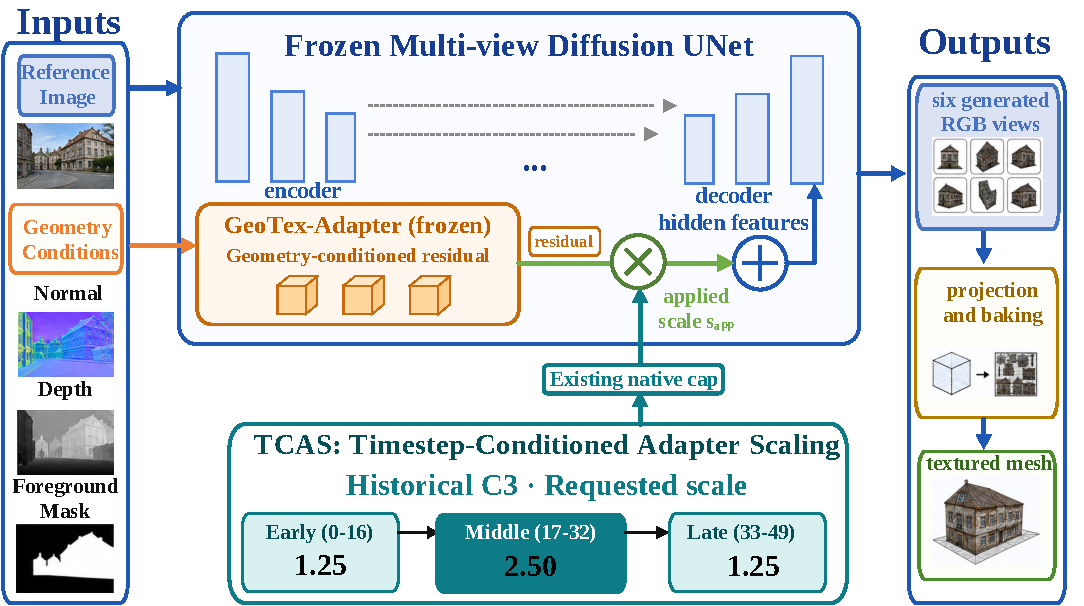
\includegraphics[width=\textwidth]{figures/fig1_tcas_control.pdf}
\caption{Overview of the TCAS control interface in multi-view diffusion texturing. The frozen pretrained GeoTex-Adapter computes geometry-conditioned residual corrections from normal, depth and foreground-mask features, together with current hidden features. TCAS specifies the historical C3 requested scaling profile (1.25, 2.50, 1.25) over steps 0--16, 17--32 and 33--49. Existing native group-specific caps determine the applied scales before residual multiplication and addition to frozen U-Net features. In the evaluated Fresh C implementation, the deep, middle and shallow caps are 3.0, 3.5 and 0.8; shallow is clipped to 0.8 throughout. Six generated RGB views can subsequently be projected and baked onto a textured mesh. The image panels are illustrative and are not used as cohort evidence.}
\label{fig:overview}
\end{figure*}

During multi-view diffusion, the 3D geometry is rendered into normal maps, depth maps, and foreground masks, denoted as:
\begin{equation}
\mathbf{G} = \{G_\text{normal}, G_\text{depth}, G_\text{mask}\}.
\end{equation}

The geometric adapter maps these conditions to a residual correction term and injects it into the intermediate hidden states of the UNet. For inference step $j$ with normalized execution progress $p_j$, the adapter injection can be written as:
\begin{equation}
\mathbf{h}'_{j,\ell} = \mathbf{h}_{j,\ell} + s_{\mathrm{app}}(p_j,\ell)\, A^\ell_\phi(\mathbf{h}_{j,\ell}, \mathbf{G}),
\label{eq:injection}
\end{equation}
Here $\ell$ identifies a wrapper within one of the three injection groups; caps and requested profiles are assigned by group. The \emph{requested scale} $s_{\mathrm{req}}(p_j,\ell)$ is the value assigned by the profile; the \emph{applied scale} is the value used by the wrapper,
\begin{equation}
s_{\mathrm{app}}(p_j,\ell)=\min\!\bigl(s_{\mathrm{req}}(p_j,\ell),c_\ell\bigr),
\end{equation}
when the native cap $c_\ell$ is active, and otherwise equals the request. The resulting correction is $\mathbf{r}_{j,\ell}=s_{\mathrm{app}}(p_j,\ell)A^\ell_\phi(\mathbf{h}_{j,\ell},\mathbf{G})$; its \emph{post-scale residual magnitude} is $m_{j,\ell}=\|\mathbf{r}_{j,\ell}\|_2$. Thus neither a requested nor an applied scale label alone determines the correction magnitude.

In the evaluated up-only Fresh C configuration, the GeoTex wrappers on UNet up blocks $\texttt{up\_0}$, $\texttt{up\_1}$ and $\texttt{up\_2}$ are assigned to the deep, middle and shallow cap groups, respectively. These names identify the implementation's grouped injection points; they do not assert universal semantic roles for denoising stages. The corresponding Fresh C caps are 3.0, 3.5, and 0.8. The shallow requests in all three C3 phases, 1.25/2.50/1.25, are applied as 0.80/0.80/0.80; deep and middle retain the requested profile. These caps belong to the existing wrapper and are not introduced by TCAS. Their values and group names do not establish causal semantic roles. GFL and GFH also clip at the shallow cap. These values describe the evaluated Fresh C wrapper; row-level cap semantics for the historical 24-object probe are not recoverable. TCAS scales a geometry residual added to feature activations; it does not reweight conditional and unconditional score predictions as classifier-free guidance does.

\subsection{Image-Space Metrics and Texture-Variation Diagnostics}
\label{subsec:metrics}

The endpoints describe different outcomes. \emph{Image-space agreement} uses target-view PSNR, LPIPS, and SSIM on the named regions; it does not measure final 3D material quality. \emph{Reference-color agreement} uses measures such as CIEDE2000 against the corresponding reference. \emph{Texture variation} uses RGB standard deviation, Laplacian variance, gradient magnitude, and high-frequency energy; these can increase with detail or artifacts and are not fidelity measures. \emph{Subjective preference} refers only to the submitted forced-choice study. \emph{Baked appearance} refers to rendered meshes after texture projection or baking, whereas \emph{PBR/material fidelity} additionally depends on the material and illumination model. These endpoints are not interchangeable: FG-SSIM, Edge-SSIM, and Crop-SSIM quantify structural similarity on named regions, PSNR measures pixel error, and LPIPS compares learned image features \cite{wang2004ssim,zhang2018lpips}. Texture-variation statistics describe local image properties; neither a higher value nor a lower one alone establishes fidelity or reference preservation.

\subsection{TCAS Control Semantics and Comparison Design}
\label{subsec:tcas}

TCAS replaces a globally fixed requested adapter scale with a piecewise profile over normalized sampling progress. The early/middle/late partition is an operational description, not a universal claim about the function of every denoising stage. C3's low--high--low profile is the recorded development choice evaluated in this study; it is not presented as an independently derived optimum.

To avoid ambiguity caused by different raw timestep directions in different schedulers, $p_j=j/(T-1)$ denotes execution progress for inference step $j\in\{0,\ldots,T-1\}$. Thus $p=0$ is the first update from the initial noisy latent and $p=1$ is the last denoising update before decoding. For $T=50$, TCAS divides execution into steps 0--16, 17--32, and 33--49 (17/16/17 steps):
\begin{equation}
s_{\mathrm{req}}(p) = \begin{cases} s_e, & 0 \leq p < 1/3 \\ s_m, & 1/3 \leq p < 2/3 \\ s_l, & 2/3 \leq p \leq 1 \end{cases}.
\label{eq:tcas}
\end{equation}

We call this variation across the 50 inference steps the \emph{temporal allocation}. A \emph{layer allocation} varies the requested scale across the three wrapper groups at a fixed step. For a schedule with applied values $s_{\mathrm{app}}(j,\ell)$, its per-group applied-scale sum is $B_\ell=\sum_j s_{\mathrm{app}}(j,\ell)$; the unweighted sum $B_{\mathrm{nom}}=\sum_\ell B_\ell$ is a \emph{nominal applied-scale budget}. It does not weight scales by adapter activations. We log post-scale correction summaries, including wrapper-level $L_2$ norm and mean absolute entry. The three wrapper groups operate on feature maps with different spatial dimensions, and the traces do not retain channel counts; raw $L_2$ values are therefore not used for cross-layer dose comparisons. The per-entry mean absolute correction reported in Supplementary Section~S1 is a dimension-normalized descriptive summary, not an equal-dose intervention. Correction magnitudes also depend on the current hidden state and earlier denoising updates, so equal nominal budgets do not imply equal realized corrections.

The selected C3 configuration used in this paper is:
\begin{equation}
(s_e, s_m, s_l) = (1.25, 2.50, 1.25).
\end{equation}

The low--high--low profile is a concrete inference-time intervention motivated by the submitted development analysis. Its stage interpretation is a task-specific hypothesis: the tested early, middle, and late allocations may produce different responses. Fresh C evaluates the recorded profile against matched controls but does not prove a universal function for any stage. TCAS adds no trained parameters and does not modify base-model or adapter weights; it replaces the requested scale during inference.

\paragraph{What C3 changes and what its comparisons identify}
C3 requests $(1.25,2.50,1.25)$ for each of the 50 steps across the three layer groups before native caps. In Fresh C, the applied deep and middle profiles retain those values; the shallow profile is clipped to 0.8 throughout. GFL requests 1.25 at every step and group, so its deep and middle values are 1.25 throughout and its shallow value is also clipped to 0.8. Their per-group applied-scale sums are therefore 82.5 versus 62.5 in deep and middle, and 40 for both in shallow. The C3--GFL contrast changes the middle-third deep/middle scale magnitude as well as its temporal allocation; it is not a timing-only comparison.

To identify a temporal-placement contrast, controls hold the per-layer applied values and nominal per-group sums fixed while moving the same values between time windows. A scale-strength contrast instead changes amplitude while preserving layer and temporal allocation. Matching requested values or applied-scale sums does not match the evolving residual corrections; raw $L_2$ values are also dimension-sensitive across wrapper groups and cannot establish cross-layer dose matching. The 300-object allocation comparison matches applied sums in each layer group and therefore estimates an allocation effect at a fixed scalar budget, not a residual-dose-independent mechanism. The historical-request sensitivity panel is reported separately.

\paragraph{Development origin and scope of C3}
The submitted study records C3 $=(1.25,2.50,1.25)$ as the selected profile from a 24-object development probe containing 17 uniform, layer-wise, and time-conditioned variants. The available historical records do not preserve the row-level outputs needed to reconstruct that ranking. We therefore treat C3 as the recorded operating point and make no optimality or uniqueness claim based on the original probe. Fresh C evaluates it without further schedule search.

\subsection{Geometry Adapter and Inference Interface}
\label{subsec:adapterimpl}

The pretrained GeoTex-Adapter receives a five-channel input comprising a three-channel normal map, a one-channel depth map, and a one-channel foreground mask. Its multi-scale encoder produces residual features that are injected into the frozen UNet. TCAS acts on the requested multiplier along denoising progress; it does not retrain the adapter, the UNet, or the VAE and introduces no learned parameters.

Visual comparisons use recorded outputs with shared object framing and crops. They illustrate task behavior and appearance limitations; quantitative conclusions use the stated object-level metrics.

\subsection{Study Cohorts, Sampling and Statistical Units}
\label{subsec:setup}

Table~\ref{tab:study-design} summarizes the cohorts and protocols. The principal evaluation cohort, denoted Fresh C, contains 300 object identities disjoint from the historical schedule-selection/evaluation pool, the recorded 1,118-object training list and the earlier clean-v2 evaluation list. Its primary four-condition comparison uses one frozen retrained GeoTex checkpoint, shared inputs and paired object seeds. This study does not reproduce the historical adapter's reported $+0.96$ dB estimate; the original main checkpoint's exact identity remains unavailable. A separate historical-request retraining is reported as protocol sensitivity.

\begin{table*}[t]
\centering\footnotesize\setlength{\tabcolsep}{3.5pt}\renewcommand{\arraystretch}{1.08}
\caption{Studies and evidence scope. Cohorts may overlap; views and seeds remain nested within object.}
\label{tab:study-design}
\begin{tabular}{p{0.16\textwidth}p{0.22\textwidth}p{0.18\textwidth}p{0.35\textwidth}}
\toprule Study / objects & Interface and sampling & Endpoint & Selection and scope \\
\midrule
Fresh C / 300 & Capped GeoTex residual; 256 px; 50 Euler steps; conditional-only & Six target-view FG metrics & UID-disjoint cohort; C3 primary; linear and matched-budget addenda \\
GeoTex bake / 10 & Controlled generator; native UVs; six bake views & Eleven unseen unlit views & Compatibility-selected pilot; Late--Mean primary; two later controls exploratory \\
MV-Adapter / 50 & Native condition-guider; 512 px; 50 steps; CFG 3 & Six native-camera views & Input-selected; thirteen legal white targets retained \\
GSO / 100 & Native MV-Adapter; 512 px; 50 steps; CFG 3; three seeds & All-six PSNR primary; nonreference LPIPS secondary & Source-ordered convenience cohort; external sensitivity \\
GSO bake / 20 & Fixed GSO inputs; native UVs; three seeds & Eleven unseen unlit views & GT-only recalibration after initial outcomes; full cohort retained \\
Reference protocol / 50 & New frozen GeoTex; native references; 512 px; CFG 2 & Five nonreference views & Previously studied inputs; protocol/checkpoint sensitivity \\
Historical request / 276 slots & Retrained GeoTex; 1,039 training UIDs; one unknown replacement & Six-view composite; full-frame and FG & Exposed technical sensitivity; exact held-out UID coverage uncertified \\
MVDiffusion / 75 & Partial correspondence-block scaling; depth unscaled & Recorded six-view endpoints & Retrospective third-interface panel; not exact GeoTex operator transfer \\
\bottomrule
\end{tabular}
\end{table*}

Within each comparison, object inputs, targets, initialization and endpoint code are shared. Fresh C uses seed $42+\texttt{object\_idx}$, held constant across conditions for that object. Its capped residual groups have deep/middle/shallow limits of 3.0/3.5/0.8. MV-Adapter uses a different feature injection operator and numerical scale range; its native target cameras and actual default-path identity are checked separately. Scale labels are not common physical doses across interfaces.

Fresh C's controlled sampler differs from the complete base pipeline, which uses online image features, classifier-free guidance and 512-pixel views. Constant 1.0 under the GeoTex caps also differs from the unset-scale residual branch. We therefore name these controls by their executed configuration. The source records and sampling/default-path diagnostics are in Supplementary Sections~S1 and S6.

FG-PSNR, LPIPS, SSIM and Edge-SSIM measure agreement on the named image regions. Baked evaluation renders actual exported meshes; unlit base color does not establish PBR or material fidelity. Fresh C image endpoints are evaluated once on each frozen $3\times2$ six-view composite. Native-interface and baked endpoints average their recorded per-view scores within object, with GSO sampling seeds also averaged within object. Paired intervals resample objects and are pointwise 95\% intervals. Preserved primary, secondary and exploratory families use their stated Holm adjustments; the distinct families do not imply one overall experiment-wide error guarantee. Non-detection is not equivalence or non-inferiority. Complete comparison rules are supplied in Supplementary Sections~S2--S5.

\paragraph{Reproducible analysis and presentation}
Statistical analyses use NumPy/SciPy with the specified object resampling, seeds and original correction families; plots use Matplotlib. The accompanying scripts and source records document the calculations and inputs for numerical verification.

\section{Experimental Results}
\label{sec:experiments}

\subsection{Competitive Controls and the Historical C3 Profile}
\label{subsec:largescale}

The internally specified Fresh C primary is C3 minus Fixed Low (GFL) FG-PSNR. The paired gain is $+0.52$ dB (95\% interval $[+0.40,+0.64]$), with 206/300 objects favorable. All conditions use the same frozen retrained checkpoint and object inputs. This gain combines increased strength and temporal allocation: C3's deep/middle applied sums are 82.5 each, versus 62.5 for GFL, while both have shallow sum 40.

\begin{table*}[t]
\centering\small\setlength{\tabcolsep}{4pt}\renewcommand{\arraystretch}{1.12}
\caption{Fresh C competitive-control means on the same 300 objects.}
\label{tab:freshc-absolute}\label{tab:matched-budget300}
\begin{tabular*}{\textwidth}{@{\extracolsep{\fill}}l S[table-format=3.2] S[table-format=2.2] S[table-format=2.2] S[table-format=1.4] S[table-format=1.4] S[table-format=1.4]}
\toprule Control & \multicolumn{1}{c}{Deep/middle sum} & \multicolumn{1}{c}{Shallow sum} & \multicolumn{1}{c}{FG-PSNR$\uparrow$} & \multicolumn{1}{c}{FG-LPIPS$\downarrow$} & \multicolumn{1}{c}{FG-SSIM$\uparrow$} & \multicolumn{1}{c}{Edge-SSIM$\uparrow$} \\
\midrule
Fixed Low & 62.5 & 40 & 11.31 & 0.2051 & 0.3500 & 0.4728 \\
Fixed High & 125.0 & 40 & 12.58 & 0.1891 & 0.4201 & 0.4961 \\
Fixed Mean & 82.5 & 40 & 11.96 & 0.1978 & 0.3864 & 0.4843 \\
Early-high & 82.5 & 40 & 11.33 & 0.2045 & 0.3696 & 0.4765 \\
C3 / Middle-high & 82.5 & 40 & 11.83 & 0.1998 & 0.3746 & 0.4773 \\
Late-high & 82.5 & 40 & 12.39 & 0.1951 & 0.3788 & 0.4914 \\
Generic Linear$^\dagger$ & 93.75 & 31.25 & 12.42 & 0.1862 & 0.4026 & 0.4880 \\

\bottomrule
\end{tabular*}
\par\smallskip
{\footnotesize Equal-budget rows (Fixed Mean, Early-high, C3/Middle-high and Late-high) share per-group sums of 82.5 for deep/middle and 40 for shallow. Generic Linear$^\dagger$ is a same-cohort addendum with different sums (93.75, 31.25); it is not an equal-budget strategy.}
\end{table*}

Competitive controls change the recommendation. Fixed High has better means than C3 on all four endpoints: C3 minus Fixed High is $-0.748$ dB FG-PSNR (pointwise interval $[-0.885,-0.609]$), with FG-SSIM difference $-0.04553$ ($[-0.04937,-0.04167]$). Generic Linear ramps deep/middle requests from 1.25 to 2.50 and shallow requests from 0.50 to 0.75 over the fifty steps. Its applied sums are (93.75,93.75,31.25), so it changes layer allocation and total budget as well as timing. It also has better means on all four; C3 minus Generic Linear is $-0.593$ dB ($[-0.837,-0.351]$). Its positive median of $+0.074$ dB and 155/300 favorable objects show why mean and object-level distributions must both be considered. Complete original paired endpoints and their comparison families are in Supplementary Section~S2.

\subsection{Temporal Allocation at Matched Applied-Scale Budgets}
\label{subsec:matched-budget300}
Early-, middle-, and late-high move the same sixteen high steps to updates 0--15, 17--32, and 34--49. Deep/middle low and high are 1.25 and 2.50; shallow stays at its 0.8 cap. Fixed Mean uses 1.65 before the cap. Each allocation therefore has per-group sums $(82.5,82.5,40)$. All six conditions share the object inputs and seed, giving 1,800 paired object-condition rows.

The equal-budget addendum's internally specified primary question is Middle-high minus the objectwise average of Early-high and Late-high FG-PSNR. Its mean is $-0.0339$ dB (10,000-resample pointwise object-bootstrap interval $[-0.1172,+0.0514]$; two-sided 20,000-draw sign-flip $p=0.4324$), with 119/300 objects positive. The median is $-0.2296$ dB. This result does not support a middle-window advantage and does not establish equivalence. It was specified before the addendum's new allocations, after earlier Fresh C outcomes were known; it is not an independent prospective confirmation. The primary, twelve-test secondary family and later descriptive all-pair analysis are distinguished in Supplementary Section~S2.

Later descriptive all-pair comparisons place Middle-high (C3) above Early-high by $+0.496$ dB and below Late-high by $-0.564$ dB in FG-PSNR; both have Holm-adjusted $p=0.00059$ in the separate retrospective 59-test family (their reported intervals are pointwise). The corresponding Middle--Early and Middle--Late FG-LPIPS differences are $-0.00472$ and $+0.00466$ (both Holm-adjusted $p=0.00059$), with the same ordering. Middle--Fixed Applied Mean FG-PSNR is $-0.133$ dB (pointwise interval $[-0.170,-0.096]$; its raw $p=0.00001$ is exempt from that family). These contrasts indicate within-cohort sensitivity to temporal placement at matched applied sums, but do not replace the specified timing primary, establish a residual-dose-independent mechanism, or validate a universally preferred late schedule. Full contrasts and family details are in Supplementary Section~S2. Within these six conditions Fixed High wins FG-PSNR on 172 objects, Late-high on 64, and C3 on none; this is an endpoint-specific count, not a universal quality ranking.

A descriptive four-endpoint comparison complements these winner counts. On 270/300 objects, at least one of the other five controls weakly dominates C3 on all four recorded composite endpoints and improves at least one. Fixed High alone does so on 173 objects, but C3 dominates it on 16; their remaining 111 objects have competing endpoints. This post-inspection, point-estimate analysis is not statistical separation on each object or a ranking of unmeasured material quality. Full counts are in Supplementary Section~S2.

The equal-budget comparison identifies an allocation total effect. Evolving residual amplitudes remain trajectory-dependent, preventing a residual-dose-independent mechanism interpretation. Late-high is not universally preferred: Fixed Mean has higher FG-SSIM, and Generic Linear is a strong unmatched-budget practical control. The historical LLH layer/time addendum and complete object distributions remain in Supplementary Section~S2.

\begin{figure*}[!t]
\centering
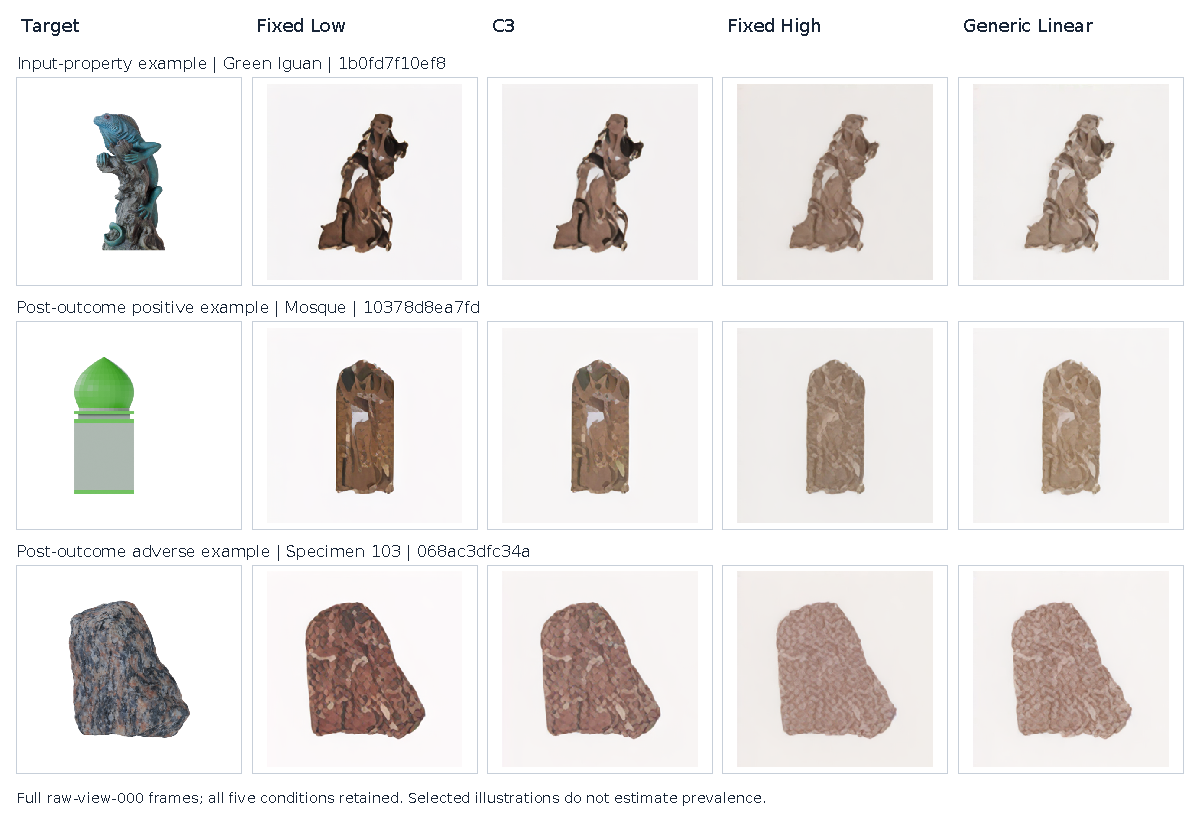
\includegraphics[width=\textwidth]{figures/fig2_freshc_controls_v4.pdf}
\caption{Fresh C, camera 000. Every row shows Target, Fixed Low, C3, Fixed High and Generic Linear in the same full-frame view. Targets are source RGB conditioning renders, not measured ground-truth albedo. Green Iguan is a colorful, textured organic object selected from source properties. Mosque ($+1.736$~dB) and Specimen 103 ($-0.468$~dB) are post-outcome selected positive and adverse C3--Fixed Low FG-PSNR examples. These selected rows illustrate endpoint heterogeneity; they do not estimate prevalence or establish a cohort-wide advantage. Complete source identity and credits are in Supplementary Section~S9 and the visual selection manifest.}
\label{fig:c3compare}
\end{figure*}


\subsection{Appearance and Color Failure Analysis}
\label{subsec:appearance-color}

The selected color diagnosis contains 26 failure-enriched objects: six earlier figure cases and 20 Fresh C panels. It is not a random sample, a new holdout, or a population estimate. No Adapter, GFL, and LLH were compared on the same inputs, checkpoint, and runner with six target views per object (78 object-condition records). The following paired object-bootstrap intervals are descriptive (20,000 resamples; seed 61008), and no confirmatory multiplicity family was defined.

\begin{table}[t]
\centering\footnotesize\setlength{\tabcolsep}{3pt}
\caption{Selected paired color-diagnostic contrasts.}
\label{tab:color-summary}
\begin{tabular*}{\columnwidth}{@{\extracolsep{\fill}}p{0.26\columnwidth}r p{0.31\columnwidth}r}
\toprule
Contrast & $\Delta E_{00}$ & 95\% CI & Favorable \\
\midrule
GFL -- No Adapter & $-19.654$ & $[-26.370,-13.248]$ & 24/26 \\
LLH -- GFL & $+3.583$ & $[+0.462,+6.712]$ & -- \\
\bottomrule
\end{tabular*}
\par\smallskip{\footnotesize Failure-enriched $N=26$; negative differences favor the first condition. Favorable is an object-direction count, not prevalence.}
\end{table}

GFL lowered reference-relative CIEDE2000 in 24/26 objects, while visible pink or purple shifts remained in two legacy examples under No Adapter, GFL, and LLH. Their mapping to the original submitted panels cannot be recovered; the Fresh C example in Figure~\ref{fig:color-failure} is a different object. The shifts are present in decoded RGB before UV projection or baking. In one case, a ground-truth VAE encode--decode isolate had CIEDE2000 4.086 and $\Delta a^*\approx-1.35$, compared with 22.032 and $+1.977$ for GFL. This weakens ordinary VAE round-trip error as the sole explanation for that example, without identifying the complete cause.

LLH--GFL increased mean CIEDE2000 while reducing foreground gradient magnitude, high-frequency energy and color entropy. Lower variation therefore did not imply closer reference appearance. The denoising/runtime isolates and three failed correction candidates remain in Supplementary Section~S6; they localize observations but do not validate a cause or repair.

Earlier bake results and calibration checks are reported separately in Supplementary Section~S5 and are not pooled with the ten-object cohort. The GeoTex residual branch with an unset scale differs from an explicit Constant 1.0 request under the wrapper caps; we label the latter by its executed setting.

\paragraph{Full-object evidence and its selection}
The complete views in Figure~\ref{fig:c3compare} and the color failure in Figure~\ref{fig:color-failure} use a shared full-frame display for every condition within each object; the existing color diagnostic retains its identical pixel crop. Favorable/adverse C3--GFL examples are retained in Supplementary Section~S9. Outcome-selected displays illustrate behavior, not prevalence. The historical texture audit does not preserve a traceable denominator or validated texture-loss labels; we therefore do not infer color-failure prevalence or texture loss from it. Variation statistics alone cannot establish fidelity.


\subsection{Actual Baked Appearance: Local Benefit and External Limits}
\label{subsec:new-bake}
\subsubsection{Native-UV protocol and primary result}
We selected ten previously unbaked Fresh C objects in UID order using input availability, native UV/material compatibility, triangle count and camera-mask alignment. Only ten of the 300 screened inputs passed these criteria before the cutoff. Their generated-view outputs were known, but their baked outcomes had not been inspected during selection. This compatibility-selected pilot is not a representative sample; five earlier bake objects are reported separately.

Seven conditions share each object's source mesh, reference, seed, six projection cameras, masks, 256-pixel source resolution, atlas resolution, hole filling and eleven unseen evaluation cameras. Original geometry and UVs are retained; unseen cameras do not enter the bake. GT-256 uses the same source resolution, masks and bake parameters, with the same raw atlas coverage as each generated condition. Camera and sampling calibrations are documented in Supplementary Section~S5. Evaluation uses unlit base color and does not measure PBR fidelity.

\begin{table}[t]
\centering\footnotesize\setlength{\tabcolsep}{2.5pt}\renewcommand{\arraystretch}{1.05}
\caption{Ten-object native-UV bake pilot: mean scores over eleven unseen views.}
\label{tab:new-bake}
\begin{tabular}{l S[table-format=2.2] S[table-format=1.4] S[table-format=1.4] S[table-format=2.2]}
\toprule Condition & \multicolumn{1}{c}{FG-PSNR} & \multicolumn{1}{c}{FG-LPIPS} & \multicolumn{1}{c}{FG-SSIM} & \multicolumn{1}{c}{CIEDE2000} \\
\midrule
GT-256 reference bake & 22.38 & 0.0590 & 0.7683 & 4.44 \\
\midrule
Native residual$^\dagger$ & 11.13 & 0.1372 & 0.3376 & 26.47 \\
No Adapter$^\dagger$ & 5.92 & 0.1600 & 0.3829 & 40.92 \\
Constant 1.0 (capped) & 11.93 & 0.1354 & 0.3504 & 24.18 \\
Fixed Low & 12.48 & 0.1317 & 0.3835 & 22.71 \\
Fixed High & 12.29 & 0.1305 & 0.4587 & 23.27 \\
Fixed Mean & 12.62 & 0.1303 & 0.4193 & 22.32 \\
C3 / Middle-high & 12.48 & 0.1302 & 0.4059 & 22.16 \\
Late-high & 12.92 & 0.1277 & 0.4259 & 21.65 \\
Generic Linear & 11.60 & 0.1276 & 0.4458 & 24.71 \\
\bottomrule\end{tabular}
\par\smallskip{\footnotesize $^\dagger$ Added exploratory controls. GT-256 is a matched reference bake, not a theoretical bound.}
\end{table}

The internally predeclared primary contrast was Late-high minus Fixed Mean on unseen-view FG-LPIPS, proposed from the earlier pilot and tested on the ten newly selected bake objects. Its mean is $-0.00265$ (95\% object-bootstrap CI $[-0.00414,-0.00137]$; exact paired sign-flip $p=0.00195$), with all ten objects favorable. This is an approximately 2.0\% reduction relative to Fixed Mean's mean LPIPS and identifies a small allocation benefit within this sampling protocol. Generic Linear has a slightly lower mean LPIPS but lower PSNR; Late-high does not dominate every endpoint or control.

\subsubsection{Reference gap and object-level effects}
The matched GT-256 reference bake has mean LPIPS 0.0590, versus 0.1303 for Fixed Mean and 0.1277 for Late-high. Post hoc, the Late-high change closes 3.7\% of the mean Fixed Mean--GT reference gap (pointwise object-bootstrap CI [2.3\%,5.3\%]). This ratio of paired means is descriptive, not a theoretical ceiling or evidence of acceptable material fidelity. Leaving out each object in turn keeps the mean Late--Mean difference between $-0.00294$ and $-0.00208$, while the substantial reference-appearance discrepancies remain. Supplementary Section~S5 provides the paired values and calculation.

C3--Fixed High has mean PSNR $+0.19$~dB (95\% CI $[-0.65,+0.87]$) and LPIPS $-0.00036$ ($[-0.00396,+0.00336]$); neither separates under the four-comparison secondary Holm family (both adjusted $p=1$). Its SSIM is lower by 0.05274 ($[-0.07459,-0.03170]$; Holm $p=0.00781$). The five-object exploratory C3 PSNR result therefore does not establish a stable benefit in this separate pilot. Late-high is a different allocation from C3.

Across the seven conditions, mean within-object Spearman correlations between generated-view and baked unseen-view rankings are 0.846 for PSNR, 0.804 for LPIPS, 0.746 for SSIM and 0.907 for Edge-SSIM. Broad rankings are positively associated, while the winning condition changes on 7/10 objects for LPIPS (1/10 for PSNR). These are different statements: we do not claim a general reversal of rankings. Figure~\ref{fig:baked-context} pairs Tire, selected by median source-foreground Laplacian variance among seven display-cleared assets, with the carved font, selected post hoc for its largest existing eleven-view LPIPS decrease. The latter also has lower PSNR, so the example displays an endpoint tradeoff rather than a general benefit. The full ten-object effect distribution and values remain in Supplementary Section~S5. These two displays illustrate persistent appearance mismatch and small, object-dependent method differences; they do not estimate prevalence or establish faithful material reproduction.

\begin{figure*}[t]
\centering
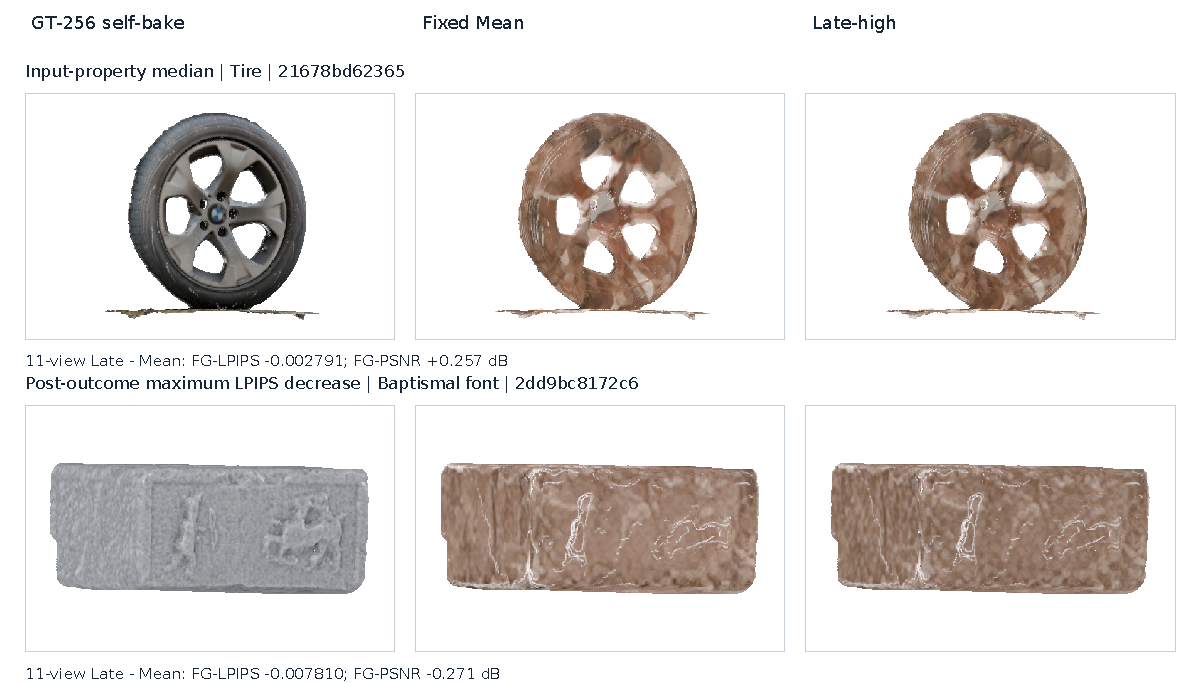
\includegraphics[width=\textwidth]{figures/fig3_bake10_two_object_v4.pdf}
\caption{GeoTex Bake10 appearance at held-out camera 004. Each row shows a GT-256 reference self-bake, Fixed Mean, and Late-high under a shared mesh/UV and within-object crop. Tire is selected by median source-foreground Laplacian variance among seven display-cleared assets. The carved font is an explicitly post-outcome example with the largest existing eleven-view Late-high minus Fixed Mean FG-LPIPS reduction among those seven ($-0.00781$); its FG-PSNR also decreases by 0.271 dB. The selected examples illustrate appearance mismatch and an endpoint tradeoff, not cohort prevalence or a general schedule benefit. Source images are 512$\times$512 and displayed without method-specific color edits. The full ten-object effect distribution and scores are in Supplementary Section~S5.}
\label{fig:baked-context}
\end{figure*}

\subsubsection{Protocol and deployment boundaries}
\paragraph{Separate twenty-object GSO evaluation}
The GSO/MV-Adapter study completes twelve conditions by three seeds on twenty fixed inputs, plus twenty matched GT self-bakes: 740 unique baked meshes and 8,140 unseen-view records. The objects, source meshes, projection cameras, texture resolution and eleven unseen cameras are shared across controls; unseen cameras do not contribute to baking.

The original twenty-object bake protocol failed a discontinuous UV-ramp diagnostic after fifteen objects. A subsequent ground-truth-only calibration addressed finite-resolution mixing across UV boundaries and retained the fixed twenty-object cohort, cameras, masks, materials and resolutions. Because this correction followed inspection of initial outcomes, the resulting GSO evaluation is reported as protocol sensitivity. The original failure and remaining UV/coverage limits are detailed in Supplementary Section~S4.

Late-high minus Fixed Mean unseen-view LPIPS is $+0.000084$ (pointwise interval $[-0.000103,+0.000286]$; original comparison-family Holm $p=0.788$). This study does not detect the ten-object pilot's benefit. It changes both input domain and conditioning/projection protocol, so it is neither a direct same-protocol replication nor evidence assigning the difference to backbone alone. Table~\ref{tab:bake-cohorts} reports the two separate bake primaries; their endpoint remains distinct from the FG-PSNR timing comparisons in Table~\ref{tab:allocation-summary}.

Supplementary Videos 1 and 2 accompany these bake studies. The GeoTex video shows two rights-cleared assets over eleven recorded unseen cameras; the GSO video shows one source-ordered object at seed 42 under twelve conditions and eleven protocol-specific cameras. The GSO source-mesh panel is not a GT self-bake. Object, camera, and display limits are detailed in Supplementary Sections~S5 and S4.

\begin{table}[t]\centering\footnotesize\setlength{\tabcolsep}{2pt}\renewcommand{\arraystretch}{1.08}
\caption{Unseen-view FG-LPIPS primary contrasts for the two bake studies.}
\label{tab:bake-cohorts}
\begin{tabular*}{\columnwidth}{@{\extracolsep{\fill}}l r p{0.39\columnwidth} r}
\toprule Study ($N$) & $\Delta$ FG-LPIPS & 95\% CI & $p$ \\
\midrule
GeoTex (10) & $-0.002652$ & $[-0.004144,-0.001367]$ & 0.00195 \\
GSO (20) & $+0.000084$ & $[-0.000103,+0.000286]$ & 0.788 \\
\bottomrule\end{tabular*}
\par\smallskip{\footnotesize Late-high minus Fixed Mean. GeoTex: exact paired sign-flip. GSO: original-family Holm16-adjusted paired sign-flip. Separate input and calibration protocols are not pooled; non-detection is not equivalence.}
\end{table}

Across all twelve GSO conditions, mean within-object image/bake LPIPS-rank correlation is 0.601 (object interval $[0.440,0.733]$). A post hoc sensitivity restricted to the seven original scale/time controls gives 0.396 ($[0.175,0.582]$), with the minimum-mean LPIPS condition changing on 11/20 objects. These are positively associated rankings with changing point-estimate winners, not general rank reversal or statistically resolved winner changes. The GT self-bake has mean LPIPS 0.0602 and PSNR 19.36 dB; average complete-bilinear-footprint coverage is about 78.7\%. All foreground remains scored and GT errors are not subtracted. These losses contextualize the small method effects without defining a theoretical quality bound.

\paragraph{Incoming-view consistency}
The bake also measures cross-camera color variance at UV texels receiving multiple source views. A constant-black control has zero variance despite its incorrect appearance, showing that this diagnostic measures incoming-view disagreement rather than fidelity. Late-high has a lower mean disagreement than Fixed Mean ($-0.002448$), while Fixed High has still lower disagreement and higher baked LPIPS. Resampling and overlapping UVs also affect this measure; it does not validate seams or PBR. Full controls and contrasts are in Supplementary Section~S5.

\paragraph{Native controls and protocol sensitivity}
Subsequently added Native residual and No Adapter outputs on the same ten GeoTex objects are exploratory. They retain matched geometry and GT coverage, and the repeated Constant 1.0 (capped) outputs are bitwise identical. Their apparent PSNR/LPIPS gains for the schedules do not separate under the fifteen-test exploratory family. The complete data are in Supplementary Section~S5.

A supporting fifty-object comparison uses a newly trained frozen GeoTex checkpoint with 512-pixel supervision, actual positive/negative reference conditions and CFG 2. Late-high minus Fixed Mean has nonreference PSNR $-1.184$ dB (interval $[-1.587,-0.849]$) and LPIPS $+0.00266$ ($[-0.00003,+0.00640]$; adjusted $p=0.080$). C3 has no corrected advantage over Fixed Mean or Fixed High. This previously studied cohort and changed checkpoint/protocol supply a sensitivity boundary, not an independent backbone confirmation. Training details and full-v29 comparisons are in Supplementary Section~S8.

\paragraph{Native-pipeline quality boundary}
The recorded full-v29 ControlNet pipeline is a stronger deployment comparator than geometry-disabled output from the new HF-based checkpoint. On the same fifty inputs and five nonreference cameras, the new geometry checkpoint trails full v29 by 2.16 dB FG-PSNR (paired interval $[-3.15,-1.27]$) and has FG-LPIPS higher by 0.0341 ($[0.0235,0.0464]$); these belong to the separately frozen four-endpoint Holm family. This is a matched-input deployment comparison, not a scale-only comparison: base weights and geometry implementations differ, and the common 50-step, seed-42, CFG-2 setting is not the official command-line default. In an exploratory follow-up that matches the exported v29 base UNet, unscaled geometry improves LPIPS over disabled geometry by 0.0131 yet remains 0.0159 worse than full v29 (paired interval $[0.0085,0.0237]$). Geometry architecture and training history still differ, and the same previously inspected objects were reused. Thus a local control benefit can coexist with a larger complete-system quality deficit; neither contrast establishes TCAS deployment superiority. Full conditions, tests and grids are in Supplementary Section~S8.

\subsection{Sensitivity Across Native Conditioning Interfaces}
\label{subsec:cross-interface}
The auxiliary studies ask related scheduling questions under different native conditioning operators and camera contracts. The 50-object and GSO100 studies both use MV-Adapter; GSO100 is a separate source-ordered cohort and protocol sensitivity, not a third independent backbone. MVDiffusion scales a partial correspondence operator and is reported only as additional context. Table~\ref{tab:allocation-summary} presents each study's own specified primary contrast: the GeoTex contrast compares Middle-high with the mean of Early-high and Late-high, whereas both MV-Adapter contrasts compare Middle-high with Fixed Mean. We report these rows separately and do not pool them or treat them as an identical replication.

\begin{figure*}[t]
\centering
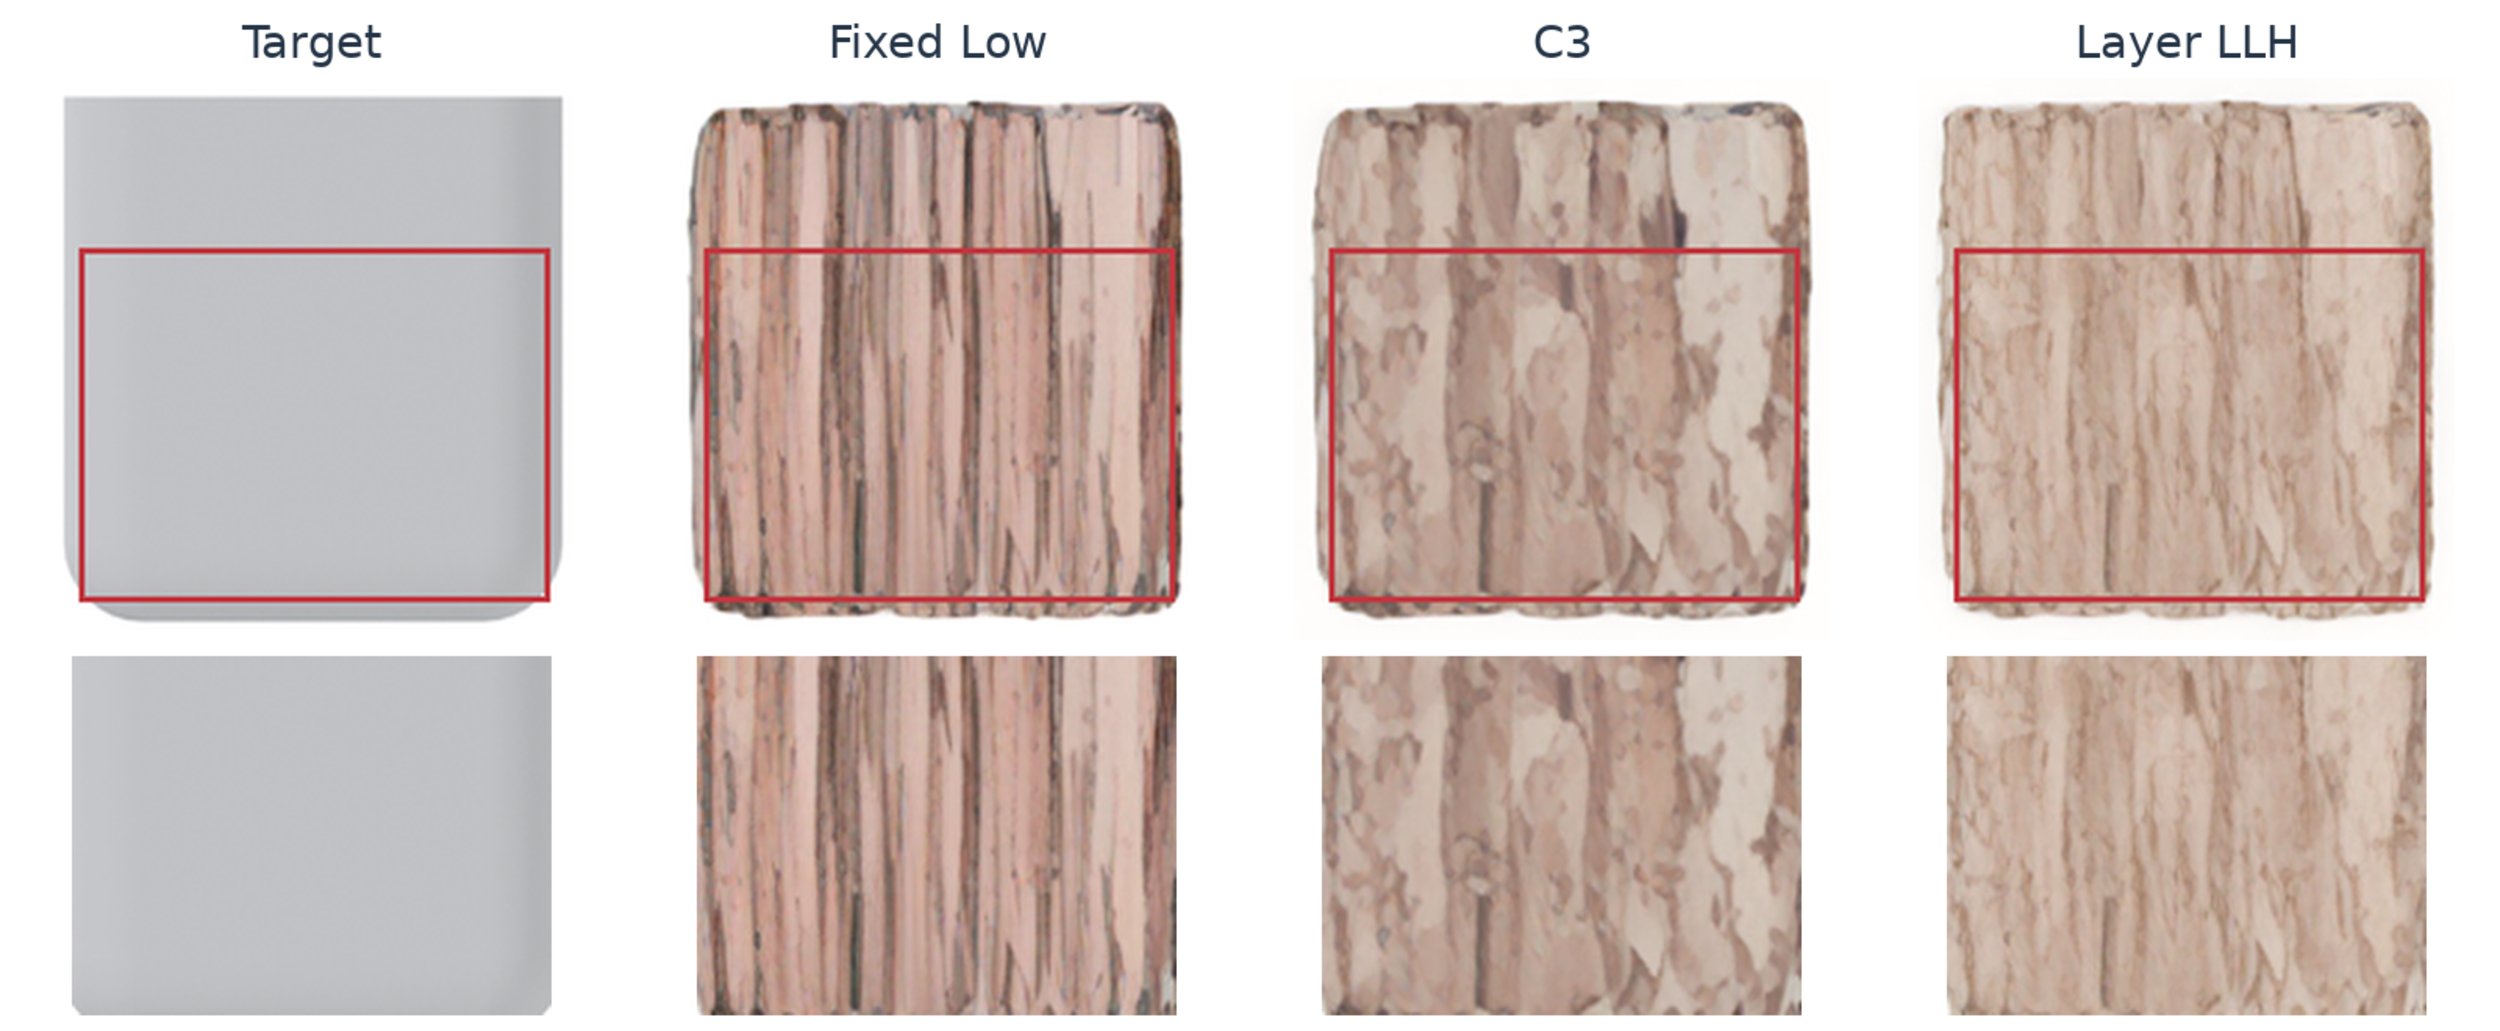
\includegraphics[width=\textwidth]{figures/fig6_color_diagnostic_freshc_context_roi.pdf}
\caption{Fresh C view 0, E5-5-2: Target, Fixed Low, C3 and layer LLH share a complete-object frame and an identical pixel crop. The generated brown pattern does not reproduce the gray target; changing its variation does not establish color fidelity. This previously viewed example came from an existing C3--GFL LPIPS stratum and was not selected for color. It does not reproduce the legacy purple-shift cases. Object credits are supplied in Supplementary Section~S9.}
\label{fig:color-failure}
\end{figure*}

\paragraph{Input-selected native MV-Adapter study}
\label{subsec:new-mva}
We selected fifty Fresh C inputs not previously evaluated through MV-Adapter, using input availability and native material/geometry compatibility. Native mesh normalization and six orthographic cameras define both generation and evaluation targets. Three-object identity checks confirmed agreement between the deployed and recorded default paths. An earlier seven-object panel had an invalid camera calibration and is excluded from these comparisons (Supplementary Section~S3).

The seven conditions share object inputs, seed, geometry and evaluation code. With 50 steps, low/high are 0.75/1.0; stage-high schedules contain 16 high steps, Fixed Mean is 0.83, and Generic Linear is 0.75--0.91. These five controls have matched per-feature sums within this interface. All 50 objects remain in the primary cohort, including thirteen texture-absent sources with legal constant-white base-color targets. Targets are unlit native-camera base color, not Fresh C's differently normalized reference renders or certified physical albedo.

\begin{table}[t]\centering\footnotesize\setlength{\tabcolsep}{2.5pt}\renewcommand{\arraystretch}{1.05}
\caption{Native-camera MV-Adapter means on fifty input-selected objects.}\label{tab:new-mva}
\begin{tabular}{l S[table-format=2.2] S[table-format=1.4] S[table-format=1.4] S[table-format=1.4]}
\toprule Condition & \multicolumn{1}{c}{FG-PSNR} & \multicolumn{1}{c}{FG-LPIPS} & \multicolumn{1}{c}{FG-SSIM} & \multicolumn{1}{c}{Edge-SSIM} \\
\midrule
Native / Fixed High & 12.60 & 0.1280 & 0.5041 & 0.3526 \\
Fixed Low & 12.73 & 0.1270 & 0.5066 & 0.3475 \\
Fixed Mean & 12.68 & 0.1279 & 0.5068 & 0.3509 \\
Early-high & 12.60 & 0.1296 & 0.5041 & 0.3503 \\
Middle-high & 12.71 & 0.1262 & 0.5061 & 0.3470 \\
Late-high & 12.74 & 0.1260 & 0.5075 & 0.3514 \\
Generic Linear & 12.72 & 0.1263 & 0.5072 & 0.3501 \\
\bottomrule\end{tabular}\end{table}

The internally predeclared primary, Middle-high minus Fixed Mean FG-PSNR, is $+0.029$~dB (95\% object-bootstrap CI $[-0.019,+0.081]$; paired Monte Carlo sign-flip $p=0.281$; 29/50 favorable). This does not support a stable middle-window gain or establish equivalence. The remaining 104 pair--metric tests use one Holm family. Middle-high has lower Edge-SSIM than Fixed Mean (adjusted $p=0.00104$); some other placement contrasts separate, including Late-high versus Early-high PSNR. Such endpoint-dependent differences do not demonstrate transferable C3 optimality. Complete contrasts, correction rules and the textured subset are in Supplementary Section~S3. This is a native-interface validation of the scheduling question, not architecture-matched replication of GeoTex's capped residual intervention.


\paragraph{Separate external-input MV-Adapter sensitivity}
The source-ordered GSO100 convenience cohort uses the same native MV-Adapter control path and three shared seeds. It includes seven scale/time profiles, with four inherited profiles frozen after earlier baseline exposure. The scheduling comparison is an external protocol sensitivity, not an independent prospective confirmation or parameter search.

The specified all-six-view Middle-high minus Fixed Mean primary is $-0.014$ dB (interval $[-0.031,+0.004]$; paired $p=0.122$). A secondary Late-high--Fixed Mean contrast is $+0.045$ dB ($[+0.024,+0.065]$; Holm83 $p=0.00335$), with SSIM $+0.00134$ (adjusted $p=0.000415$). Its five-nonreference-view LPIPS difference is $-0.000086$ ($[-0.000551,+0.000413]$; separate Holm21 $p=1$). Thus a small detected image effect does not establish a perceptual or baked-appearance benefit. Table~\ref{tab:allocation-summary} reports the original Fresh C timing primary first, followed by the two study-specific native-interface FG-PSNR primaries; Table~\ref{tab:bake-cohorts} retains the separate bake LPIPS primaries. Full paired secondary families remain in Supplementary Sections~S3--S5. The complete rights-cleared native-camera comparison across all seven MV-Adapter conditions is retained in Supplementary Section~S3.

\begin{table*}[t]\centering\footnotesize\setlength{\tabcolsep}{5pt}\renewcommand{\arraystretch}{1.16}
\caption{Study-specific FG-PSNR schedule primaries.}
\label{tab:allocation-summary}
\begin{tabular*}{\textwidth}{@{\extracolsep{\fill}}l l r r l r}
\toprule Study & Contrast & $N$ & $\Delta$ FG-PSNR (dB) & 95\% CI (dB) & $p$ \\
\midrule
GeoTex Fresh C & Middle $-$ mean(Early, Late) & 300 & $-0.033877$ & $[-0.117170,+0.051422]$ & 0.432378 \\
MV-Adapter50 & Middle $-$ Fixed Mean & 50 & $+0.028986$ & $[-0.019411,+0.080739]$ & 0.280747 \\
GSO100 & Middle $-$ Fixed Mean & 100 & $-0.013660$ & $[-0.030565,+0.003519]$ & 0.122279 \\
\bottomrule
\end{tabular*}
\par\smallskip{\footnotesize Middle/Early/Late denote the corresponding high-window allocations. GeoTex tests Middle against mean(Early,Late); each MV-Adapter study tests Middle against Fixed Mean. GSO100 uses the same MV-Adapter backbone as the 50-object study. Pointwise paired-object intervals; equal applied sums do not imply equal realized residual dose.}
\end{table*}

\paragraph{Fixed-seed sensitivity}
A post-inspection analysis retains all three recorded sampling seeds. GSO100 Late--Mean PSNR averages are positive at each seed ($+0.057,+0.038,+0.039$ dB), but only 27/100 objects improve at all three and 68/100 have mixed or tied directions. Its nonreference LPIPS averages change direction ($-0.000389,-0.000269,+0.000398$). For the GSO20 bake, only 1/20 objects has lower Late--Mean LPIPS at all three seeds; 14/20 have mixed or tied directions. Sign agreement has no practical-effect threshold. These conditional, object-level summaries do not estimate training randomness or revise the original primary tests; full seed intervals and deltas are in Supplementary Section~S4.

The retrospective 75-object MVDiffusion panel scales correspondence-block outputs rather than the GeoTex residual operator. Its layer-wise L--LLH condition is worse than global fixed low in PSNR, structural agreement and reference-color error; LPIPS does not separate. This result and the earlier MV-Adapter panel remain in Supplementary Section~S3 and delimit the scope of cross-interface transfer.

Projection-guidance candidates are retained as exploratory negative results in Supplementary Sections~S4 and S8; they do not form a validated alternative method.

\subsection{Historical Cohort Sensitivity and Prior Evaluation}
\label{subsec:original276}

The 276-slot retraining is a protocol/checkpoint sensitivity panel on a previously exposed request list. Seventy-nine requested UIDs overlapped the recorded training list; removing them left 1,039 training UIDs. An empty input at requested slot 46 triggered a random replacement whose UID was not recorded, so the 1,104 rows do not verify 276 distinct held-out objects. C3 minus Fixed High is $+1.699$ dB in full-frame PSNR (all 276 slots positive) but $-1.314$ dB in FG-PSNR (9/276 favorable), with FG-LPIPS higher by 0.01127, FG-SSIM lower by 0.05961, and Edge-SSIM lower by 0.02777. Excluding the known failed slot preserves the opposing PSNR means ($+1.697$ and $-1.311$ dB) and LPIPS loss ($+0.01127$); white-background normalization also favors Fixed High. C3 exceeds Fixed Low by 0.783 dB FG-PSNR, while their descriptive LPIPS interval includes zero. Fixed Mean, moved high windows, and Generic Linear were not tested, so this panel cannot identify a schedule effect or reproduce the historical $+0.96$ dB result. The slot means, paired endpoints, and unknown-UID limitation remain documented in Supplementary Section~S7.

The original blinded 3AFC study reports a 58.1\% overall-quality share for C3 (two-level participant/object-bootstrap interval $[50.1,65.8]\%$) on its own thirty-object stimuli and twenty-four participants. It does not measure the retrained checkpoint's texture fidelity or unseen baked appearance. Historical FAC re-examinations reduced FG-PSNR relative to TCAS, but the reported training pools differ (1,706 versus 1,200 objects) and seed, checkpoint, and sampled-run records are incomplete. These results remain historical context; counts, source identity, recovered code, and validation limits are in Supplementary Section~S7.


\FloatBarrier
\section{Discussion and Limitations}
\label{sec:limitations}

\paragraph{Why nominal control schedules can mislead}
The principal contribution is an evidence chain from the executed residual interface to generated views and the final textured asset, rather than a new schedule parameterization. This distinction matters because C3's gain over Fixed Low changes both strength and timing: the deep and middle applied-scale sums rise from 62.5 to 82.5, while the shallow requests are clipped to the same 0.8 value. Fixed High and Generic Linear have better means than C3 across all four image endpoints. With per-group applied sums matched, the specified Middle-high contrast is $-0.0339$ dB (95\% interval $[-0.1172,+0.0514]$), providing no detected middle-window advantage. A separate retrospective all-pair family distinguishes Middle-high from Early-high and Late-high in both FG-PSNR and FG-LPIPS, indicating placement sensitivity within this cohort. Equal scalar sums still allow the adapter activations and hidden-state trajectory to change, so these contrasts identify an allocation effect at matched nominal budget, not a residual-dose mechanism or a universally preferred late schedule. Reporting the actual cap-adjusted intervention and testing strong alternatives therefore changes how the original C3 result should be interpreted.

\paragraph{What survives texture baking}
Generated-view and baked-view rankings are positively associated in the GeoTex pilot, but projection and texture construction remain consequential: point-estimate winners can change between endpoints. On ten compatibility-selected objects, Late-high reduces unseen-view LPIPS by $0.00265$ (about 2\% relative to Fixed Mean) and closes 3.7\% of the reference self-bake gap. This is a small local asset-level effect beside substantial remaining appearance error, not a texture-quality upper bound or evidence of faithful material reproduction. The separate GSO20 bake study does not detect the same benefit after a calibration change made following initial outcome inspection; its different cohort and protocol prevent treating it as a direct replication. Likewise, the new geometry checkpoint trails full v29 by 2.16 dB FG-PSNR and has FG-LPIPS higher by 0.0341 under a recorded non-default matched-input comparison. Because weights and geometry implementations differ, this marks a deployment-quality boundary rather than a schedule effect. Unlit base-color renders and incoming-view variance do not establish PBR fidelity, seams, or physical albedo.

\paragraph{Interface and object dependence}
The native MV-Adapter50 and GSO100 primaries do not detect their specified middle-window contrasts, but their comparators differ from the GeoTex timing primary, and GSO100 uses the same MV-Adapter interface rather than an independent backbone. MVDiffusion tests only a partial correspondence operator. These studies delimit transfer across implementations; they do not form one pooled or architecture-matched replication. A retrospective FRESH\_CONFIRM\_300 analysis also associates foreground texture variation with the LLH--Fixed Low response (Laplacian-variance Spearman $\rho=-0.524$; quartile mean effects $+4.140,+1.127,-0.087,-0.029$ dB). That association identifies a candidate source of response heterogeneity, not a causal texture effect, threshold, or adaptive schedule. Together, these results give graphics researchers a reason to report the interface, camera contract, and object-level asset response when evaluating geometry-control allocation.

\paragraph{Practical implications and limitations}
For a texturing system, the evidence supports comparing the deployed control with strong within-interface settings, reporting requested and applied profiles, and evaluating shared-mesh bakes from unseen cameras against a matched reference self-bake. It does not justify replacing a deployed fixed setting with C3 or selecting Late-high universally. The bake cohorts are compatibility-selected, the GSO calibration followed initial outcomes, and the matched-budget analysis is retrospective on an already evaluated cohort. Fresh C uses controlled retraining rather than an authenticated historical main checkpoint; the 276-slot panel includes an unknown replacement UID and does not verify distinct held-out coverage. Human preference applies only to its original stimuli, historical FAC checkpoints are incomplete, and three fixed seeds do not estimate training variation. These constraints limit replication and transfer while leaving the paired within-protocol results interpretable; detailed records remain in Supplementary Sections~S6--S8.

\section{Conclusion}
\label{sec:conclusion}

We evaluated geometry-control allocation from its implemented GeoTex residual interface through image generation and native-UV texturing. On 300 held-out objects, stronger fixed and linear controls revise the interpretation of C3's gain over Fixed Low, while the specified matched-budget primary detects no middle-window advantage. Baking shows a small Late-high unseen-view LPIPS improvement on ten compatible objects alongside substantially larger reference-appearance error; a separate bake protocol does not detect the same benefit. These findings make the graphics contribution an implementation-aware, asset-level evaluation of control allocation, rather than a new universal scheduling method. They support comparing applied controls with strong alternatives and measuring the textured asset from unseen views, without identifying a universally preferred schedule or establishing faithful material reproduction.

\section*{Data availability}

The accompanying research package contains object-level metrics, frozen protocols and configuration records, analysis scripts, and the LaTeX source needed to rebuild the manuscript and Supplement. Recovered FAC source is supplied with a record of its entry points and validation scope; these component checks do not constitute a historical full-model replay. Statistical summaries can be recomputed without model weights, while fresh inference requires the recorded weights, runtime and licensed source assets. Raw generated-image archives, trained checkpoints and participant-level responses are not included. Source assets must be acquired under their recorded licenses. Additional analysis records may be requested from the corresponding author, subject to licensing, privacy and archive constraints.

\section*{Declaration of competing interests}

The authors declare that they have no known competing financial interests or personal relationships that could have appeared to influence the work reported in this paper.


\begingroup
\linespread{0.94}\selectfont
\begin{thebibliography}{45}
\bibitem{liu2023zero1to3}
Liu R, Wu R, Van Hoorick B, et al. Zero-1-to-3: Zero-shot one image to 3D object. \textit{Proceedings of the IEEE/CVF International Conference on Computer Vision}, 2023.

\bibitem{shi2023zero123pp}
Shi R, Chen H, Zhang Z, et al. Zero123++: A single image to consistent multi-view diffusion base model. arXiv:2310.15110, 2023.

\bibitem{liu2023syncdreamer}
Liu Y, Lin C, Zeng Z, et al. SyncDreamer: Generating multiview-consistent images from a single-view image. \textit{International Conference on Learning Representations}, 2024.

\bibitem{long2023wonder3d}
Long X, Guo Y C, Lin C, et al. Wonder3D: Single image to 3D using cross-domain diffusion. \textit{Proceedings of the IEEE/CVF Conference on Computer Vision and Pattern Recognition}, 2024.

\bibitem{shi2024mvdream}
Shi Y, Wang P, Ye J, et al. MVDream: Multi-view diffusion for 3D generation. \textit{International Conference on Learning Representations}, 2024.

\bibitem{wang2023imagedream}
Wang P, et al. ImageDream: Image-prompt multi-view diffusion for 3D generation. arXiv:2312.02201, 2023.

\bibitem{xu2024instantmesh}
Xu J, et al. InstantMesh: Efficient 3D mesh generation from a single image with sparse-view large reconstruction models. \textit{Advances in Neural Information Processing Systems}, 2024.

\bibitem{ke2024era3d}
Li P, Liu Y, Long X, et al. Era3D: High-resolution multiview diffusion using efficient row-wise attention. \textit{Advances in Neural Information Processing Systems}, 2024.

\bibitem{chen2023text2tex}
Chen D Z, et al. Text2Tex: Text-driven texture synthesis via diffusion models. \textit{Proceedings of the IEEE/CVF International Conference on Computer Vision}, 2023.

\bibitem{richardson2023texture}
Richardson E, Metzer G, Alaluf Y, et al. TEXTure: Text-guided texturing of 3D shapes. \textit{ACM SIGGRAPH 2023 Conference Proceedings}, 2023.

\bibitem{poole2023dreamfusion}
Poole B, Jain A, Barron J T, Mildenhall B. DreamFusion: Text-to-3D using 2D diffusion. \textit{International Conference on Learning Representations}, 2023.

\bibitem{chen2023fantasia3d}
Chen R, Chen Y, Jiao N, Jia K. Fantasia3D: Disentangling geometry and appearance for high-quality text-to-3D content creation. \textit{Proceedings of the IEEE/CVF International Conference on Computer Vision}, 2023.

\bibitem{shao2025mvpainter}
Shao M, Xiong F, Sun Z, Xu M. MVPainter: Accurate and detailed 3D texture generation via multi-view diffusion with geometric control. arXiv:2505.12635, 2025.

\bibitem{kynkanniemi2024limited}
Kynk\"a\"anniemi T, Aittala M, Karras T, et al. Applying guidance in a limited interval improves sample and distribution quality in diffusion models. \textit{Advances in Neural Information Processing Systems}, 2024.

\bibitem{perla2026survey}
Perla S R K, Zhang H, Mahdavi-Amiri A. Advances in neural 3D mesh texturing: A survey. \textit{Computer Graphics Forum}, 2026, e70392.

\bibitem{guzman2026adaptive}
Guzm\'an J E, Mould D, Paquette E. Adaptive multiresolution exemplar-based texture synthesis on animated fluids. \textit{Computers \& Graphics}, 2026, 134: 104490.

\bibitem{lv2025interpretable}
Lv X, Wu Z, Xu J, et al. Interpretable procedural material graph generation via diffusion models from reference images. \textit{The Visual Computer}, 2025, 41(13): 11195--11205.

\bibitem{zeng2024paint3d}
Zeng X, Chen X, Qi Z, et al. Paint3D: Paint Anything 3D with Lighting-Less Texture Diffusion Models. \textit{Proceedings of the IEEE/CVF Conference on Computer Vision and Pattern Recognition}, 2024.

\bibitem{cheng2024mvpaint}
Cheng W, Mu J, Zeng X, et al. MVPaint: Synchronized multi-view diffusion for painting anything 3D. \textit{Proceedings of the IEEE/CVF Conference on Computer Vision and Pattern Recognition}, 2025.

\bibitem{lai2025hunyuan3d}
Zhao Z, Lai Z, Lin Q, et al. Hunyuan3D 2.0: Scaling diffusion models for high resolution textured 3D assets generation. arXiv:2501.12202, 2025.

\bibitem{huang2024mvadapter}
Huang Z, et al. MV-Adapter: Multi-view consistent image generation made easy. \textit{Proceedings of the IEEE/CVF International Conference on Computer Vision}, 2025.

\bibitem{tang2023mvdiffusion}
Tang S, Zhang F, Chen J, Wang P, Furukawa Y. MVDiffusion: Enabling holistic multi-view image generation with correspondence-aware diffusion. \textit{Advances in Neural Information Processing Systems}, 2023.

\bibitem{liu2024synchronized}
Liu Y X, Xie M S, Liu H Y, Wong T T. Text-guided texturing by synchronized multi-view diffusion. \textit{SIGGRAPH Asia 2024 Conference Papers}, 2024.

\bibitem{xu2026wondertex}
Xu Q, Han X G, Zhang L. WonderTex: Consistent-and-seamless texture generation with text-guided multi-view image diffusion models. \textit{IEEE Transactions on Visualization and Computer Graphics}, 2026, 32(7): 5815--5825.

\bibitem{mou2023t2iadapter}
Mou C, Wang X, Xie L, et al. T2I-Adapter: Learning adapters to dig out more controllable ability for text-to-image diffusion models. \textit{Proceedings of the AAAI Conference on Artificial Intelligence}, 2024.

\bibitem{zhang2023controlnet}
Zhang L, Rao A, Agrawala M. Adding conditional control to text-to-image diffusion models. \textit{Proceedings of the IEEE/CVF International Conference on Computer Vision}, 2023.

\bibitem{ye2023ipadapter}
Ye H, Zhang J, Liu S, Han X, Yang W. IP-Adapter: Text compatible image prompt adapter for text-to-image diffusion models. arXiv:2308.06721, 2023.

\bibitem{hu2022lora}
Hu E J, Shen Y, Wallis P, et al. LoRA: Low-rank adaptation of large language models. \textit{International Conference on Learning Representations}, 2022.

\bibitem{liu2024dora}
Liu S Y, Wang C Y, Yin H, et al. DoRA: Weight-decomposed low-rank adaptation. \textit{International Conference on Machine Learning}, 2024.

\bibitem{zhang2023adalora}
Zhang Q, Zuo S, Liang C, et al. AdaLoRA: Adaptive budget allocation for parameter-efficient fine-tuning. \textit{International Conference on Learning Representations}, 2023.

\bibitem{kulkarni2026ssi}
Kulkarni A S. Scheduled Style Injection: Expanding the Style-Content Pareto Frontier in Training-Free Diffusion-Based Style Transfer. \textit{Proceedings of the IEEE/CVF Conference on Computer Vision and Pattern Recognition Workshops (CVPRW), NTIRE Workshop}, 2026.

\bibitem{ho2020ddpm}
Ho J, Jain A, Abbeel P. Denoising diffusion probabilistic models. \textit{Advances in Neural Information Processing Systems}, 2020.

\bibitem{song2021ddim}
Song J, Meng C, Ermon S. Denoising diffusion implicit models. \textit{International Conference on Learning Representations}, 2021.

\bibitem{ho2022cfg}
Ho J, Salimans T. Classifier-free diffusion guidance. \textit{NeurIPS Workshop on Deep Generative Models and Downstream Applications}, 2021. arXiv:2207.12598.

\bibitem{castillo2023adaptive}
Castillo A, Kohler J, P\'erez J C, et al. Adaptive guidance: Training-free acceleration of conditional diffusion models. \textit{Proceedings of the AAAI Conference on Artificial Intelligence}, 2025.

\bibitem{wang2004ssim}
Wang Z, Bovik A C, Sheikh H R, Simoncelli E P. Image quality assessment: From error visibility to structural similarity. \textit{IEEE Transactions on Image Processing}, 2004, 13(4): 600--612.

\bibitem{zhang2018lpips}
Zhang R, Isola P, Efros A A, et al. The unreasonable effectiveness of deep features as a perceptual metric. \textit{CVPR}, 2018.

\bibitem{sad2024apg}
Sadat S, Hilliges O, Weber R M. Eliminating oversaturation and artifacts of high guidance scales in diffusion models. \textit{International Conference on Learning Representations}, 2025.

\bibitem{chung2024styleid}
Chung J, Hyun S, Heo J P. Style Injection in Diffusion: A Training-free Approach for Adapting Large-scale Diffusion Models for Style Transfer. \textit{Proceedings of the IEEE/CVF Conference on Computer Vision and Pattern Recognition}, 2024.

\bibitem{controlnet2023layercontrol}
ControlNet project. Official depth-to-image demo: layer-dependent control scales. Source code, fixed commit f2e1bc38dc8d925fb542be4c138c46013ace1988, 2023. \url{https://github.com/lllyasviel/ControlNet/blob/f2e1bc38dc8d925fb542be4c138c46013ace1988/gradio_depth2image.py}. Accessed 12 October 2026.

\bibitem{diffusers2023controlnet}
Hugging Face. Diffusers v0.21.0: ControlNet conditioning scale and guidance start/end. Official versioned documentation, 2023. \url{https://huggingface.co/docs/diffusers/v0.21.0/api/pipelines/controlnet}. Accessed 12 October 2026.

\end{thebibliography}
\endgroup
\end{document}
